\documentclass[11pt, a4paper]{article}
\usepackage{mwe}
\usepackage{amsmath, amssymb}
\usepackage{mathtools}
\usepackage{graphicx}
\graphicspath{{"../figures/"}}
\usepackage[section]{placeins} % to keep figures in their sections
\usepackage[export]{adjustbox} % for subcaptionbox figures

\usepackage{xcolor}
\usepackage{bm} % for bold vectors in math mode
\usepackage{physics} % for differential notation, etc...
\usepackage[separate-uncertainty=true]{siunitx}

\usepackage[most, minted]{tcolorbox} % for displaying code

\newtcblisting{myminted}{%
	listing engine=minted,
	minted language=python,
	listing only,
	breakable,
	enhanced,
	minted options = {
		linenos, 
		breaklines=true, 
		tabsize=2,
		fontsize=\footnotesize, 
		numbersep=2mm
	},
	overlay={%
		\begin{tcbclipinterior}
			\fill[gray!25] (frame.south west) rectangle ([xshift=4mm]frame.north west);
		\end{tcbclipinterior}
	}   
}

\usepackage[margin=3cm]{geometry}
\usepackage[colorlinks = true,
            linkcolor = blue,
            urlcolor  = blue,
            citecolor = blue,
            anchorcolor = blue]{hyperref}

\setlength{\parindent}{0pt} % to stop indenting new paragraphs
\newcommand{\diff}{\mathop{}\!\mathrm{d}} % differential
\newcommand{\eqtext}[1]{\qquad \text{#1} \qquad}
\newcommand{\mat}[1]{\mathbf{#1}}
\renewcommand{\vec}[1]{\bm{#1}}



\newcommand{\lev}{L\'evy\xspace}
\newcommand{\mad}{\operatorname{MAD}}


\begin{document}
\title{Random Walks}
\author{Elijan Jakob Mastnak\\[1mm]\small{Student ID: 28181157}}
\date{October 2020}
\maketitle

\tableofcontents


\newpage


\begin{center}
\textbf{Assignment}
\end{center}
Create a computer simulation of two-dimensional random walks and random flights. Start at the origin ($ x = y = 0 $), and determine the next position by randomly choosing an independent direction $ \phi $ and step size $ l $, i.e.
\begin{equation*}
	x_{n+1} = x_{n} + l \cos \phi \eqtext{and} y_{n+1} = y_{n} + l \sin \phi
\end{equation*}
where $ \phi $ is uniformly distributed on the interval $ [0, 2\pi) $ and $ l $ is distributed according to $ p(l) \propto l^{-\mu} $. Plot a few examples of walks and flights for 10, 100, 1000, and 10000 steps. From a large number of walks/flights, each with a large number of steps, determine the value of the exponent $ \gamma $ for a few chosen values of the parameter $ \mu $ and use this result the characterize each walk/flight by its diffusion regime.

%\textbf{Optional:} Additionally, randomly vary the sticking time between individual steps according to the power distribution $ p(t) \propto t^{-\nu} $ where $ 1 < \nu < 2 $. Is the sticking time dependence uncoupled from the distribution of the elementary walk/flight over the lengths/times of individual steps?

\rule{\textwidth}{0.2pt}


\section{Theory}
\vspace{-2mm}
\textit{To jump right to the solution, see \hyperref[randwalk:s:solution]{Section \ref{randwalk:s:solution}}}.
\vspace{3mm}

Random walks are a form of motion in which, over a process of many individual steps, a ``walker'' (e.g. a point particle) progresses from the origin to some final position while the parameters of each step (e.g. size, direction) randomly change over the course of the walk. 

\subsection{Normal Diffusion}
Diffusion---net movement of particles from high to low concentration---can be modeled by treating each particle as a random walker. In \textit{normal diffusion}, a particle's final position averaged over a large number of random walks, denoted by $ \expval{r(t)} $, tends to stay at the origin, while variance of the final distance from the origin over time, denoted by $ \sigma_{r}^{2}(t) $, grows linearly with walk time as:
\begin{equation*}
	\sigma_{r}^{2}(t) \equiv \big\langle r^{2}(t) \big\rangle - \big\langle r(t) \big\rangle^{2} = 2Dt
\end{equation*}
The proportionality constant $ D $ is the \textit{diffusion constant}. As long as the mean time between steps and mean squared step size are finite, the central limit theorem states that the resulting distribution of final distances from the origin follows a normal distribution.

\subsection{Anomalous Diffusion} 
We now consider random walks with a possibility of very large step sizes, and parameterize the step length distribution's probability density function with the power distribution
\begin{equation}
	p(l) \propto l^{-\mu} \label{randwalk:eq:step-size-distribution}
\end{equation}
where $ \mu \in (1, 3) $. In this case, the distribution's second moment 
\begin{equation*}
	\expval{l^{2}} = \int_{0}^{\infty} l^{2} p(l) \diff l
\end{equation*}
diverges, and the central limit theorem does not apply. In this case, the variance $ \sigma_{r}^{2}(t) $ behaves as
\begin{equation}
	\sigma_{r}^{2}(t) \sim t^{\gamma} \label{randwalk:eq:anomalous-variance}
\end{equation}
where the value of the exponent $ \gamma $ depends on the value of $ \mu $ in Equation \ref{randwalk:eq:step-size-distribution}. Diffusion with a non-linear relationship between $ \sigma_{r}^{2} $ and $ t $ is called \textit{anomalous diffusion}. We will consider two types of anomalous diffusion: \lev flights and \lev walks.


\subsubsection{\lev Flights}
\lev flights are a subset of anomalous diffusion in which each step takes the same amount of time. Because the time of each step is fixed and step size, determined by Equation \ref{randwalk:eq:step-size-distribution}, can vary wildly, so too can the speed at which steps are taken. The flight's total time is directly proportional to the total number of steps.

\vspace{2mm}
\textit{Summary: Fix step time, draw random step size, adjust step speed to match step time.}
\vspace{2mm}


For \lev flights, the theoretically expected relationship between $ \gamma $ and $ \mu $ is
\begin{equation}
	\gamma(\mu) = 
	\begin{cases}
		\frac{2}{\mu - 1} & \mu \in (1, 3) \qquad (\text{super-diffusion})\\
		1 & \mu > 3 \qquad \quad \ \ (\text{normal diffusion})
	\end{cases} \label{randwalk:eq:flight-gamma}
\end{equation}
The special case $ \mu = 2 $ gives $ \gamma = 2 $, which is called \textit{ballistic diffusion.}

\subsubsection{\lev Walks}
\lev walks are a subset of anomalous diffusion in which each step is taken at the same fixed speed. Because the step speed is fixed and step size, determined by Equation \ref{randwalk:eq:step-size-distribution}, can vary wildly, so too do the times each step takes---the time each step takes is proportional to the step size. The time of the entire walk is proportional to the total distance traveled.

\vspace{2mm}
\textit{Summary: Fix step speed, draw random step size, adjust step time to match step speed.}
\vspace{2mm}



For \lev walks, the expected relationship between $ \gamma $ and $ \mu $ is
\begin{equation}
	\gamma(\mu) = 
	\begin{cases}
		2 & \mu \in (1, 2) \qquad (\text{ballistic diffusion})\\
		4 - \mu & \mu \in (2, 3) \qquad (\text{super-diffusion})\\
		1 & \mu > 3 \qquad \quad \ \ (\text{normal diffusion})
	\end{cases} \label{randwalk:eq:walk-gamma}
\end{equation}
For the special cases $ \mu = 2 $ and $ \mu = 3 $ we expect
\begin{equation*}
	\mu = 2 \implies \sigma_{r}^{2}(t) \sim \frac{t^{2}}{\ln t} \eqtext{and} \mu = 3 \implies \sigma_{r}^{2}(t) \sim t \ln t
\end{equation*}


\iffalse
I generate $ l $ using the concept of inverse transformation sampling, which assumes the cumulative distribution function's values are monotonically increasing and bounded in the interval $ [0, 1] $. Instead of finding a closed-form expression for the inverse cumulative distribution function. Instead, I left stuff in integral form. To sample a value of the random variable $ X $, distributed according to the distribution $ w(x) $, from the interval $ [a, b] $, 
\begin{equation*}
	\int_{a}^{x}w(\chi)\diff \chi = \rho \cdot \int_{a}^{b}w(\chi) \diff \chi
\end{equation*}
$ \rho $ is a (pseudo) random number uniformly distributed on the interval $ [0, 1] $. 
\fi

\iffalse
\subsection{Statistical Note}
For anomalous diffusion of the form Equation \ref{randwalk:eq:step-size-distribution} where the second moment $ \langle l \rangle^{2} $ diverges, calculating the variance $ \sigma_{r}^{2} $ of $ N $ final positions $ \{r_{n}\} $ using the definition
\begin{equation*}
	\sigma_{r}^{2} = \frac{1}{N-1}\sum_{n=1}^{N}\big(r_{n} - \expval{r}\big)^{2}
\end{equation*}
won't work well. The standard deviation is highly sensitive to outliers (i.e. very large step sizes) and will tend to either diverge or vary wildly between simulations. 

It is better to use robust statistics to analyze the spread of the set $ \{r_{n}\} $. For example median absolute deviation ($ \mad $), defined for a set $ \{R_{i}\} $ as
\begin{equation*}
	\mad \equiv \operatorname{median}_{i}\big (\abs{R_{i} - \operatorname{median}_{j}R_{j}}\big)
\end{equation*}
\fi

\iffalse
\textbf{Normalization:} As for any properly behaving probability density function, $ p(l) $ in Equation \ref{randwalk:eq:step-size-distribution} must be normalized. This is impossible over the entire real line for $ \mu \in (1, 3) $, but if we sample from $ l $ from $ l_{\text{min}}, l_{\text{max}} \subset (0, \infty) $, then $ p(l) $ can be normalized.
\begin{equation*}
	p(l) = C l^{-\mu} \eqtext{where} \frac{1}{C} = \int_{l_{\text{min}}}^{l_{\text{max}}} l^{-\mu}\diff l = \frac{1}{1-\mu}\left(l_{\text{max}}^{1-\mu} - l_{\text{min}}^{1-\mu}\right)
\end{equation*}
In practice, the normalization constant would cancel from both sides of the equation when finding $ l $. 
\fi

\section{Solution} \label{randwalk:s:solution}

\subsection{Random Number Generation}
As suggested in the instructions, I modeled a random step in two dimensions using polar coordinates: an angle $ \phi \in [0, 2\pi] $ controlling direction and a length $ l \in (\epsilon, \infty) $ controlling step size. Here $ \epsilon $ denotes a small quantity; I personally used $ \epsilon = 10^{-5} $, but the exact value is not critical and only serves to set the problem's distance scale.

\subsubsection{Sampling Angle}
I sampled the angle $ \phi $ uniformly from the interval $ [0, 2\pi] $ with a simple call to a pseudo-random number generation function, in my case the NumPy Python library's \texttt{random.uniform} function. Mathematically, the relevant equation is
\begin{equation}
	\phi = \rho_{\phi} \cdot 2 \pi \label{randwalk:eq:phi-generation}
\end{equation}
where $ \rho_{\phi} $ is a (pseudo) random number uniformly distributed on the interval $ [0, 1] $. In practice, I just used \texttt{np.random.uniform(0, 2*np.pi)}, which achieves the same result.

\subsubsection{Sampling Step Size}
I sampled step length $ l $ according to the power distribution in Equation \ref{randwalk:eq:step-size-distribution} from the interval $ (\epsilon, \infty) $ using the generating function
\begin{equation*}
	l(\rho_{l}) = \epsilon \cdot (1 - \rho_{l})^{\frac{1}{1-\mu}}
\end{equation*}
where $ \rho_{l} $ is pseudo-random number uniformly distributed on $ [0, 1] $. 

\vspace{1mm}
\textit{Derivation:} Start with the inverse transformation sampling-motivated equation
\begin{equation*}
	\int_{l_{\text{min}}}^{l}p(t)\diff t = \rho_{l} \cdot \int_{l_{\text{min}}}^{l_{\text{max}}}p(t) \diff t \eqtext{or} \int_{l_{\text{min}}}^{l}t^{-\mu}\diff t = \rho_{l} \cdot \int_{l_{\text{min}}}^{l_{\text{max}}} t^{-\mu} \diff t
\end{equation*}
Solving the integrals, inserting the integration limits and solving for $ l $ leads to
\begin{equation*}
	\eval{\frac{t^{1-\mu}}{1-\mu}}_{t=l_{\text{min}}}^{l} =  \eval{\frac{\rho_{l} \cdot  t^{1-\mu}}{1-\mu}}_{t=l_{\text{min}}}^{l_{\text{max}}} \implies l = \left[(1 - \rho_{l}) \cdot l_{\text{min}}^{1-\mu}+ \rho_{l} \cdot l_{\text{max}}^{1-\mu}\right]^{\frac{1}{1-\mu}}
\end{equation*}
As $ l_{\text{min}} \to \epsilon $ and $ l_{\text{max}} \to \infty $, the $ l_{\text{max}}^{1-\mu} $ term grows negligibly small compared to $  l_{\text{min}}^{1-\mu} $, leaving
\begin{equation}
	l = \left[(1 - \rho_{l}) \cdot \epsilon^{1-\mu}\right]^{\frac{1}{1-\mu}} =  \epsilon \cdot (1 - \rho_{l})^{\frac{1}{1-\mu}} \label{randwalk:eq:l-generation}
\end{equation}
See \href{https://www.desmos.com/calculator/jnvmt1mseb}{\underline{this Desmos link}} for an interactive example of $ l(\rho) $, showing the results of changing the parameters $ l_{\text{min}} $ and $ \mu $.

\vspace{2mm}
A simple Python function for generating $ \phi $ and $ l $ might read
\begin{myminted}
import numpy as np
l_min, mu = 1e-5, 2.      # set minimum step size and mu
np.random.seed(42)        # seed the random number generator

def phi_l_sampling_example():
    phi = np.random.uniform(0, 2*np.pi)    # samples phi from (0, 2pi)
    rho = np.random.uniform(0, 1)          # random float on (0, 1)
    l = l_min * (1 - rho) ** (1/(1 - mu))  # generates power-distributed step size
    return phi, l
\end{myminted}
\vspace{1mm}
\textbf{Important:} For a proper random walk, $ \phi $ and $ l $ must be \textit{independent}, meaning the values of the random number $ \rho $ used to generate them must be drawn separately. I tried to highlight this with the notation $ \rho_{\phi} $ and $ \rho_{l} $ (instead of using just $ \rho $ for both $ \phi $ and $ l $).




\subsubsection{Random Step Algorithm} \label{randwalk:sss:random_step_algorithm}
To generate a single random step, I sampled a random $ \phi $ and $ l $ according to Equations \ref{randwalk:eq:phi-generation} and \ref{randwalk:eq:l-generation} and increment the walker's $ x $ and $ y $ positions according to
\begin{equation*}
	x_{n + 1} \to x_{n} + l \cos \phi \eqtext{and} y_{n + 1} \to y_{n} + l \sin \phi
\end{equation*}
Note that a walker's next position depends only the previous position but is otherwise memory-less. For bookkeeping purposes, I also increment walk time either by the fixed step time $ t_{0} $ (for \lev flights) or by $ l/v_{0} $ (step length divided by fixed step speed; for \lev walks) and increment step number $ n $.

A simple code implementation---adaptable to either flights or walks---might read:
\begin{myminted}
t0, v0 = 1, 1   # step parameters for Levy flights and walks, respectively
def get_next_step_example(x, y, t, n): # input x, y, time and step number
    phi, l = phi_l_sampling_example()  # generate random phi and l
    x_step = l * np.cos(phi)           # calculate increments to x and y
    y_step = l * np.sin(phi)
    x = x + x_step                     # update x and y positions
    y = y + y_step
    if(flight): t += t0                # increment time by fixed step time
    if(walk): t += l / v0              # increment time by using fixed speed
    n += 1                             # increment step number
    return x, y, t, n
\end{myminted}

\subsection{Simulating an Entire Flight and Walk} \label{randwalk:ss:walk simulation}
For the record, my walk parameters are $ l_{\text{min}} = 10^{-5} $, $ v_{0} = 1 $ for walks and $ t_{0} = 1 $ for flights, chosen for a one-to-one correspondence between elapsed flight time and step number.

\vspace{2mm}
\textbf{\lev Flight}\\[1mm]
Simulating a \lev flight is simple: decide on the number of steps in the walk and generate that many steps using the random step algorithm above. For example:
\begin{myminted}
def get_levy_flight(n_steps):
    x, y, t, n = 0, 0, 0, 0  # initialize position, time and step number
    x_list, y_list, r_list, t_list = np.zeros(n_steps), np.zeros(n_steps), np.zeros(n_steps), np.zeros(n_steps)  # arrays to hold flight history
    for i in range(0, n_steps):
        x, y, t, n = get_next_flight_step(x, y, t, n)  # generate steps
        x_list[i] = x
        y_list[i] = y
        r_list[i] = np.sqrt(x ** 2 + y ** 2)
        t_list[i] = t
    return x_list, y_list, r_list, t_list
\end{myminted}
\textbf{My (Perhaps Ill-Fated) Approach to \lev Walks}\\[2mm]
I tried experimenting with a different approach here. Namely: setting a fixed total walk time rather than a fixed number of steps. Here is my thought process: as far as I understand, the eventual goal is to find the variance in $ r $ as a function of \textit{time}, not as a function of step number. If I simulate walks for a fixed number of steps, the total time of each walk will vary, which complicates calculating variance across all walks at a given time. Simulating walks for a fixed time instead of a fixed number of steps simplifies this, explained further in \hyperref[randwalk:sss:walk-MAD-explanation]{Subsubsection \ref{randwalk:sss:walk-MAD-explanation}}. However---skipping ahead somewhat---this approach to \lev walks may be responsible for the deviation of the fitted parameter $ \gamma $ from the theoretically expected value in the super-diffusive regime, shown in Figure \ref{randwalk:fig:walk-fit}.

\vspace{2mm}
Following is an example Python function for generating a \lev walk:
\begin{myminted}
def get_levy_walk(walk_time):
    x, y, t, n = 0, 0, 0, 0  # initialize position, time and step number
    x_list, y_list, r_list, t_list = [], [], [], []  # to hold flight history
    while t < walk_time:  # simulate for given time, not given step number
        x, y, t, n = get_next_walk_step(x, y, t, n)  # generate steps
        x_list.append(x)
        y_list.append(y)
        r_list.append(np.sqrt(x ** 2 + y ** 2))
        t_list.append(t)
    return x_list, y_list, r_list, t_list, n
\end{myminted}


\subsection{Plots of Random Walk and Flight}
To avoid cluttering the main report with too many figures---\LaTeX{} is somewhat finicky with float placement---I moved the plots of 2D random walks and flights to \hyperref[randwalk:s:2D-walk-plots]{Appendix \ref{randwalk:s:2D-walk-plots}}, where you will find plots of both \lev flights and walks in the ballistic, super-diffusive and normal regimes for 10, 100, 1000 and 10000 steps. \hyperref[randwalk:s:3D-walk-plots]{Appendix \ref{randwalk:s:3D-walk-plots}} shows analogous plots in three dimensions.

\subsection{MAD Calculation} \label{randwalk:ss:MAD-calculation}
This section quantifies the spread in the walkers' distance from the origin over time. Although mean squared displacement $ \sigma_{r}^{2} $ is standard in the literature, I used median absolute deviation ($ \mad $), which proves better suited to the large outlying values of $ r $. 

\subsubsection{MAD Calculation for \lev Flights} \label{randwalk:sss:flight-MAD-explanation}
Here is the procedure I used to calculate $ \mad $ for \lev flights:
\begin{itemize}
	\item Simulate $ N_{\text{flight}} $ flights, each with $ N_{\text{step}} $ steps. For each flight, call the flight simulation function in \hyperref[randwalk:ss:walk simulation]{Section \ref{randwalk:ss:walk simulation}}, which returns distance from origin $ r $ at each step. Because steps correspond one-to-one with time, this data is equivalent to distance from the origin at each time $ t $. I used $ N_{\text{flight}} = 10^{4} $ and $ N_{\text{step}} = 10^{3}$. 
	
	\item Create a distances matrix $ \mat{R} $ with dimensions $ (N_{\text{steps}} \cross N_{\text{walks}}) $ whose columns are the $ r(t) $ lists for each walk.
	
	\item Calculate MAD of the $ \mat{R} $ matrix across rows using \texttt{stats.median\_abs\_deviation(R, axis=1)}. This gives the flight's $ \mad $ as a function of time. In Python:
\end{itemize}

\begin{myminted}
def flight_simulation_example(n_walks, n_steps):
    r_matrix = np.zeros((n_steps, n_walks))  # matrix of distances from origin
    for i in range(0, n_walks):
        _, _, r, _, _ = get_levy_flight(n_steps)  # list of x, y, r, time and n for each walk. Only r is needed here
        r_matrix[:, i] = r  # sets the walk r as the r_matrix's ith column
    r_mad = stats.median_abs_deviation(r_matrix, axis=1)  # takes MAD across rows
    t = np.linspace(1, t0*n_steps, n_steps)  # take advantage of fixed step time
    return t, r_mad
\end{myminted}

\subsubsection{MAD Calculation for \lev Walks} \label{randwalk:sss:walk-MAD-explanation}
Here is the somewhat involved procedure I used to calculate $ \mad $ for \lev walks:
\begin{itemize}
	\item Simulate $ N_{\text{walk}} $ walks each of fixed duration $ t_{\text{walk}} $. For each walk, call the flight simulation function in Section \ref{randwalk:ss:walk simulation}, which returns distance from origin $ r $ versus time.
	
	As for \lev flights, I used $ N_{\text{walk}} = 10^{4}$. Because of the varying step number in each walk, I could not fix a single value for $ N_{\text{step}} $, but instead chose $ t_{\text{walk}} $ so that the median number of steps per walk was about $ 10^{3} $, as for \lev flights.
	
	\item Calculate median number of steps $ N_{\text{med}} $ per walk (I used median instead of mean to mitigate the effect of outlying step numbers). 
	
	Create a distance matrix $ \mat{R} $ with $ N_{\text{med}} $ rows and $ N_{\text{walk}} $ columns and a time list vector $ \bm{t}_{\text{med}} \in \mathbb{R}^{N_{\text{med}}} $ with $ N_{\text{med}} $ entries spaced uniformly from $ 0 $ to $ t_{\text{walk}} $.  
	
	\item For each walk, loop through each time in $ \bm{t}_{\text{med}} $, and assign the walker's position $ r $ at that time to the corresponding entry in $ \mat{R} $. This step takes advantage of the fact that $ \bm{t}_{\text{med}} $ and each simulated walk have the same time duration (even though the number of steps vary) and both grow monotonically from the initial to the final time.
	
	The result is a distance matrix $ \mat{R} $ with a uniform number of entries per column for each walk characterizing the walkers' distance from the origin over time.
	
	\item At this point, proceed as for flights: calculate MAD of the $ \mat{R} $ matrix across rows to find the walk's $ \mad $ as a function of time.
\end{itemize}
I'm leaving out the code---which is either tedious array index manipulation or identical to the flight case---since I don't think it adds any extra value to the above explanation.


\subsection{Determining Gamma with Linear Regression}
The parameter $ \gamma $ and the $ \mad_{r}(t) $ data are connected by the proportionality chain
\begin{equation*}
	\mad_{r}^{2}(t) \propto \sigma_{r}^{2}(t) \propto t^{\gamma} \implies \mad_{r}^{2}(t) = \alpha t^{\gamma}, \quad \alpha \in \mathbb{R}
\end{equation*}
This power relationship begs for log linearization! Taking the logarithm of both sides gives
\begin{equation*}
	2 \ln\big[\mad_{r}(t)\big] = \gamma \ln(t) + \ln(\alpha),
\end{equation*}
meaning the power $ \gamma $ is the slope of the best-fit line passing through the quantity $ 2 \ln\big[\mad_{r}(t)\big] $ plotted on the ordinate axis versus $ \ln(t) $ plotted on the abscissa. To find $ \gamma $, I calculated the $ \mad_{r}(t) $ for various values of the parameter $ \mu $ as described in \hyperref[randwalk:ss:MAD-calculation]{Subsection \ref{randwalk:ss:MAD-calculation}} for both flights and walks, linearized the data as described above, and used the \texttt{SciPy} library's \texttt{curve\_fit} function to perform the linear regression. \texttt{curve\_fit} also returns a covariance matrix whose diagonal entries give an estimate of the error on the fit parameters.  \hyperref[randwalk:ss:error]{Subsection \ref{randwalk:ss:error}} explains how I estimated the error of each $ 2 \ln\big[\mad_{r}(t)\big] $ data point.

\vspace{2mm}
\hyperref[randwalk:fig:flight-fit]{Figures \ref{randwalk:fig:flight-fit}} and \ref{randwalk:fig:walk-fit} show the fitted values of $ \gamma $, including an estimate of error, for three regimes of \lev flights and walks, respectively.

\begin{figure}
	\centering
	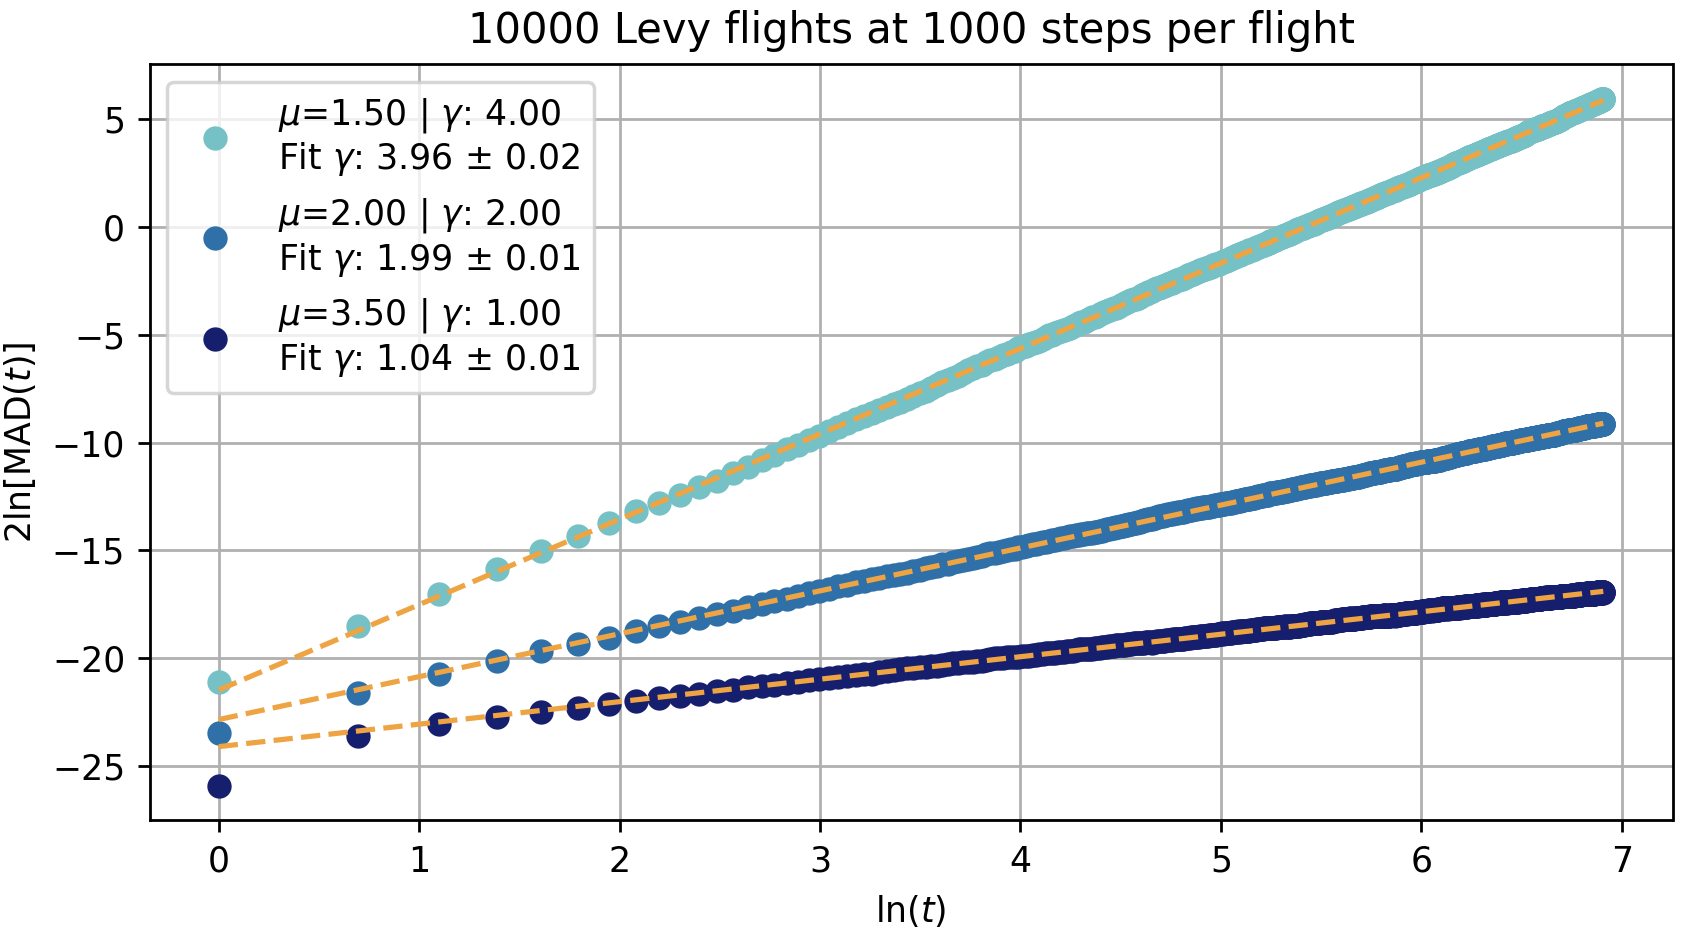
\includegraphics[width=\linewidth]{flight-fit}
	\caption{Finding the parameter $ \gamma $ for three regimes of \lev flights using linear regression. The legend compares the theoretically expected and fitted value for each $ \mu $. In order of increasing $ \mu $, the flights fall in the super-diffusive, ballistic, and normal regimes. Error is estimated using the regression's corresponding covariance matrix.}
	\label{randwalk:fig:flight-fit}
\end{figure}


\begin{figure}
	\centering
	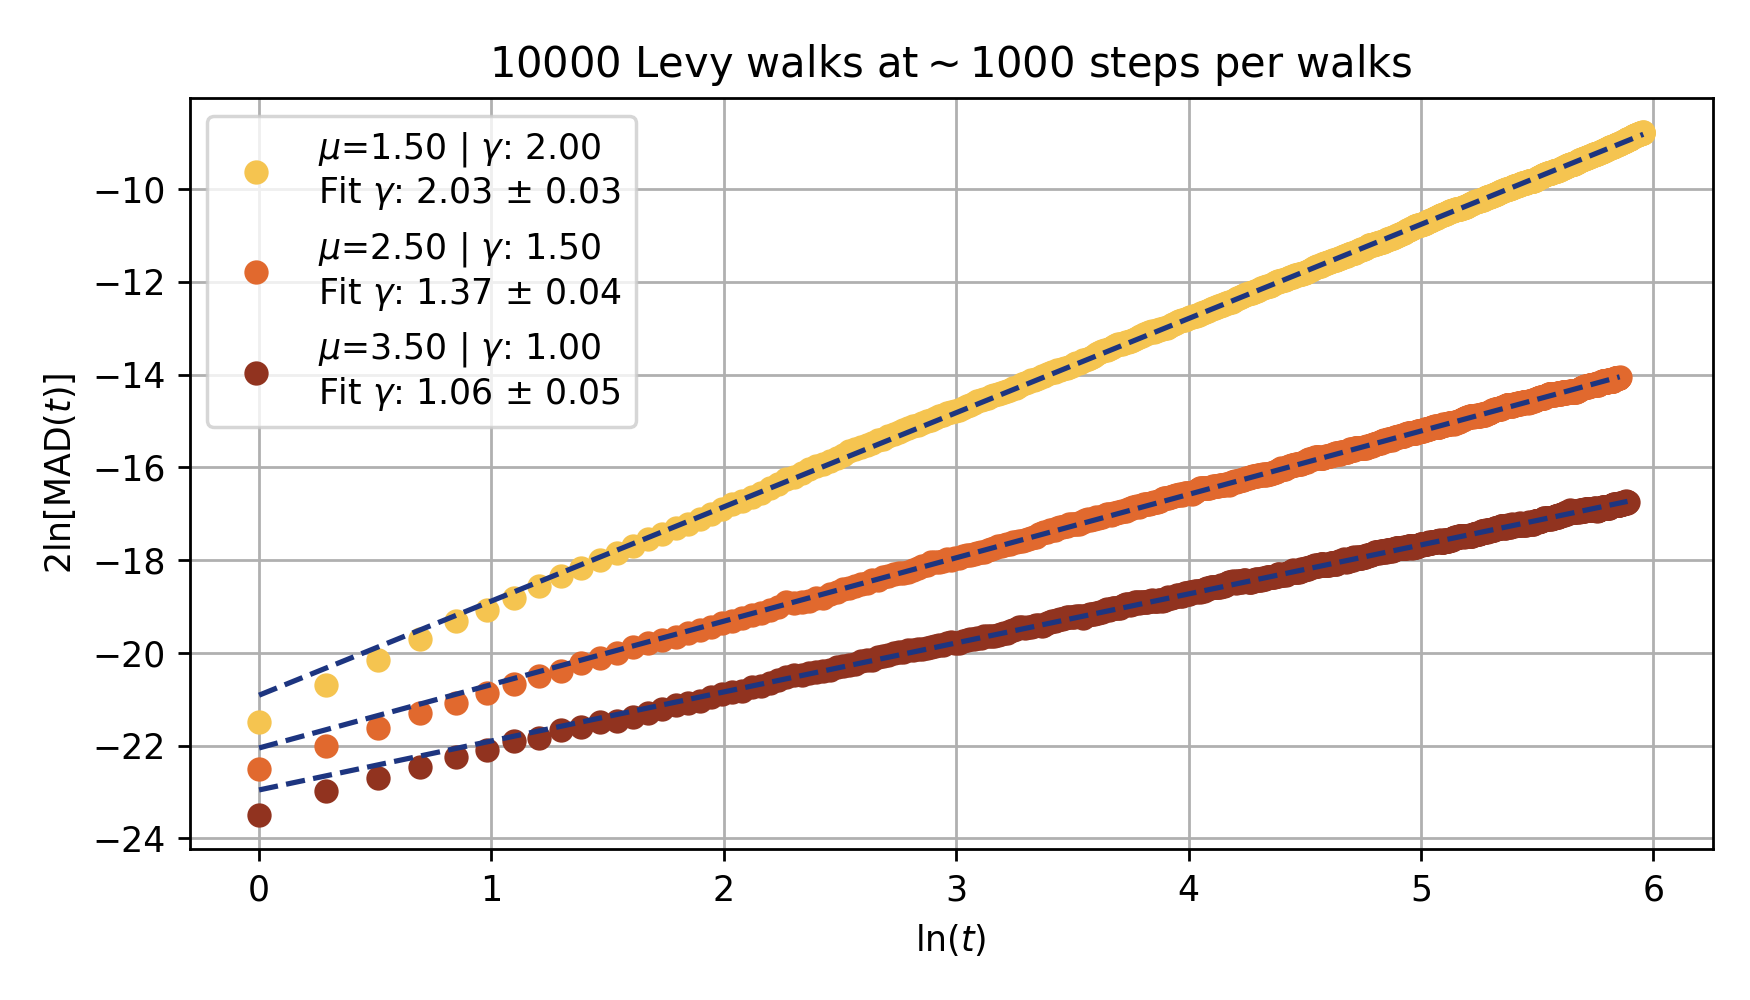
\includegraphics[width=\linewidth]{walk-fit}
	\caption{Finding the parameter$ \gamma $  for three regimes of \lev walks using linear regression. The legend compares the theoretically expected and fitted value for each $ \mu $. In order of increasing $ \mu $, the walks fall in the ballistic, super-diffusive, and normal regimes. Error is estimated using the regression's corresponding covariance matrix. Note that time values have been shifted so all three graphs are next to each other, which gives a better visual presentation without changing the lines' slopes.}
	\label{randwalk:fig:walk-fit}
\end{figure}

\vspace{2mm}
\textbf{Discussion of Results}
\begin{itemize}
	\item I believe the simulation of \lev flights and subsequent ``extraction'' of $ \gamma $ is satisfactory. The fitted values of $ \gamma $ closely agree with the theoretically expected values---to within less than one percent for $ \mu = 1.5 $ and $ 2.0 $ and a somewhat larger four percent error for $ \mu = 3.5 $ in the normal diffusion regime---and agree with the theoretical values within the realm of the regression error.
	
	\item Meanwhile, the \lev walks are somewhat lacking. On the one hand, in the ballistic and normal regimes ($\mu = 1.5$ and $ 3.5 $) the fitted values of $ \gamma $ more or less agree with the theoretically expected values within the range of regression error. On the other hand, (even though the discrepancy is not drastic) the fitted value of $ \gamma $ differs appreciably from the theoretically predicted value in the super-diffusive $ \mu = 2.5 $ case. I imagine the problem lies in my approach to handling the varying-step nature of \lev walks when calculating $ \mad_{r}(t) $, discussed in \hyperref[randwalk:sss:walk-MAD-explanation]{Subsubsection \ref{randwalk:sss:walk-MAD-explanation}}.
	
\end{itemize}


\subsection{Estimating Error of Individual Data Points} \label{randwalk:ss:error}
This section explains how I estimated the error on each $ 2 \ln\big[\mad_{r}(t)\big] $ data point when performing linear regression. Note that there's probably a better way to do this---the approach feels a bit ``hacky'', but is at least an honest attempt if nothing else.

In essence, I assumed the quantity $ 2 \ln[\mad_{r}(t)] $ behaved as a random variable distributed about a central value, so that its standard deviation provided an estimate of its error. To realize this idea:
\begin{itemize}
	\item For each value of $ \mu $, I ran 50 sets of 100 walks at either 1000 steps per walk (for \lev flights) or at a fixed time corresponding to about 1000 median steps per walk (for \lev walks). Of course, I changed the random seed at each run. I calculated the $ \mad_{r}(t) $ values of each run as described in Subsections \ref{randwalk:sss:flight-MAD-explanation} and \ref{randwalk:sss:walk-MAD-explanation}.
	
	\item I found $ 2 \ln[\mad_{r}(t)] $ from $ \mad_{r}(t)  $ and then calculated the sample standard deviation of the 50 resulting $  2 \ln[\mad_{r}(t)] $ values at each point in time. The choice of 50 runs is somewhat arbitrary; I just needed a large enough number for the concept of standard deviation to become meaningful. 
	
	\item I used the sample standard deviation $ s $ as an estimate of the standard error $ \sigma $ at each time $ t $. These values gave an estimate of the error of $  2 \ln[\mad_{r}(t)]  $ as a function of time. In this way each point is assigned an individual error, rather than just assuming a blanket error for all points.
	

\end{itemize}
Given the large number of runs, I simulated only 100 walks per set when estimating error (instead of 10000 when estimating $ \gamma $) because of finite computing power. I then assumed error scaled by a factor of $ \sqrt{\frac{100}{10000}} $ in accordance with square root statistics when scaling up from 100 to 10000 walks per simulation, since more walks corresponds to more samples.


\appendix
\section{Plots of Random Walks in 2D} \label{randwalk:s:2D-walk-plots}
This section includes plots of \lev flights and walks in the ballistic, super-diffusive and normal regimes for 10, 100, 1000 and 10000 steps. The progression in color gradient from light to dark corresponds to increasing step number and is intended to help visualize the walk's time evolution.

Two fairly obvious observations:
\begin{enumerate}
	\item The walks in the anomalous diffusion regime are dominated by the large steps, while the walks in the normal diffusion regime are more ``balanced''.
	
	\item The plots exhibit a fractal-like nature as the number of steps increases. This trend is particularly visible in the anomalous diffusion cases.
\end{enumerate}


\begin{figure}
	\centering
	{\includegraphics[width=\linewidth]{{2dflight-mu-2.0}.png}}\vfill
	{\includegraphics[width=\linewidth]{{2dwalk-mu-1.5}.png}}
\end{figure}

\begin{figure}
	\centering
	{\includegraphics[width=\linewidth]{{2dflight-mu-2.5}.png}}\vfill
	{\includegraphics[width=\linewidth]{{2dwalk-mu-2.5}.png}}
\end{figure}

\begin{figure}
	\centering
	{\includegraphics[width=\linewidth]{{2dflight-mu-3.5}.png}}\vfill
	{\includegraphics[width=\linewidth]{{2dwalk-mu-3.5}.png}}
\end{figure}


\section{Plots of Random Walks in 3D} \label{randwalk:s:3D-walk-plots}
This section is included just for fun---basically an excuse to play around with \texttt{matplotlib}'s 3D plotting capabilities. I generated the random steps as described in e.g. \hyperref[randwalk:sss:random_step_algorithm]{Subsubsection \ref{randwalk:sss:random_step_algorithm}}, but scaled to three-dimensional spherical coordinates by including a polar angle $ \theta $ uniformly distributed on $ [0, \pi] $. 
\vspace{-4mm}

\begin{figure}[H]
	\centering
	{\includegraphics[width=0.8\linewidth]{{3dflight-mu-2.0}.png}}\vfill
	{\includegraphics[width=0.8\linewidth]{{3dwalk-mu-1.5}.png}}
\end{figure}

\begin{figure}
	\centering
	{\includegraphics[width=\linewidth]{{3dflight-mu-2.5}.png}}\vfill
	{\includegraphics[width=\linewidth]{{3dwalk-mu-2.5}.png}}
\end{figure}

\begin{figure}
	\centering
	{\includegraphics[width=\linewidth]{{3dflight-mu-3.5}.png}}\vfill
	{\includegraphics[width=\linewidth]{{3dwalk-mu-3.5}.png}}
\end{figure}


\end{document}



